% ============================================================
%  護你安 HuYouAn — 期末報告簡報
%  Compiler: XeLaTeX  |  Theme: Metropolis
% ============================================================
\documentclass[aspectratio=169,12pt]{beamer}

\usepackage{fontspec}
\usepackage{xeCJK}
\setCJKmainfont{Noto Sans CJK TC}
\setCJKsansfont{Noto Sans CJK TC}
\setCJKmonofont{Noto Sans CJK TC}

% ── Metropolis theme ────────────────────────────────────────
\usetheme[progressbar=frametitle,block=fill]{metropolis}

\definecolor{mprimary}{RGB}{18,53,91}      % deep navy
\definecolor{maccent}{RGB}{231,76,60}      % red-orange
\definecolor{msuccess}{RGB}{39,174,96}     % green
\definecolor{mlightbg}{RGB}{245,246,250}   % off-white

\setbeamercolor{normal text}{fg=mprimary!90!black,bg=white}
\setbeamercolor{frametitle}{bg=mprimary,fg=white}
\setbeamercolor{progress bar}{fg=maccent,bg=mprimary!30}
\setbeamercolor{alerted text}{fg=maccent}
\setbeamercolor{example text}{fg=msuccess}
\setbeamercolor{block title}{bg=mprimary,fg=white}
\setbeamercolor{block body}{bg=mlightbg,fg=mprimary!90}
\setbeamercolor{block title alerted}{bg=maccent,fg=white}
\setbeamercolor{block body alerted}{bg=maccent!10,fg=mprimary!90}
\setbeamercolor{block title example}{bg=msuccess,fg=white}
\setbeamercolor{block body example}{bg=msuccess!10,fg=mprimary!90}
\setbeamercolor{palette primary}{bg=mprimary,fg=white}
\setbeamercolor{structure}{fg=mprimary}

\setbeamertemplate{frame numbering}[fraction]

% ── Packages ────────────────────────────────────────────────
\usepackage{tikz}
\usetikzlibrary{shapes.geometric,arrows.meta,positioning,calc,fit}
\usepackage{booktabs}
\usepackage{tabularx}
\usepackage{multirow}
\usepackage{listings}
\usepackage{graphicx}
\usepackage{array}
\usepackage{colortbl}
\usepackage{pifont}
\newcommand{\cmark}{\ding{51}}

% ── Listings ────────────────────────────────────────────────
\lstset{
  basicstyle=\ttfamily\tiny,
  keywordstyle=\color{mprimary}\bfseries,
  commentstyle=\color{gray!70},
  stringstyle=\color{maccent},
  breaklines=true,
  frame=none,
  backgroundcolor=\color{mprimary!6},
  xleftmargin=4pt, xrightmargin=4pt,
  aboveskip=2pt, belowskip=2pt,
}

% ── TikZ styles ─────────────────────────────────────────────
\tikzset{
  svc/.style={rectangle,rounded corners=5pt,draw=#1!60,fill=#1!12,
    text width=2.5cm,align=center,minimum height=0.85cm,
    font=\small\bfseries,text=#1!80!black},
  arr/.style={-{Stealth[length=5pt]},thick,draw=#1!70},
  dbtbl/.style={rectangle,draw=mprimary!50,fill=mprimary!7,
    rounded corners=3pt,text width=3.0cm,align=left,font=\scriptsize},
}

% ── Meta ────────────────────────────────────────────────────
\title{護你安 HuYouAn}
\subtitle{Employee Safety \& Response System\\雲原生應用程式開發 114-2 期末報告}
\author[第三組]{%
  \textbf{第三組} \quad
  江彥宏 \enspace 葉又銘 \enspace 彭麒任 \enspace 廖振翔 \enspace 林彥穎}
\date{2026}
\institute{}

% ============================================================
\begin{document}
% ============================================================

\maketitle

\begin{frame}{目錄}
  \setbeamertemplate{section in toc}[sections numbered]
  \tableofcontents[hideallsubsections]
\end{frame}

% ============================================================
\section{系統簡介}
% ============================================================

\begin{frame}{問題與解法}
\begin{columns}[T,onlytextwidth]
\begin{column}{0.47\textwidth}
  \begin{alertblock}{！\enspace 痛點}
    \begin{itemize}\small
      \item 緊急事件發生（地震、火災、資安）時，\textbf{傳統人工聯繫}效率低、易遺漏
      \item 管理者無法即時掌握\textbf{全員安全狀態}
      \item 跨部門回報鏈長，資訊傳遞延遲
    \end{itemize}
  \end{alertblock}
\end{column}
\hfill
\begin{column}{0.47\textwidth}
  \begin{exampleblock}{\cmark\enspace 解法}
    \begin{itemize}\small
      \item \textbf{自動化、即時}的緊急安全回報系統
      \item 員工一鍵回報安全狀態
      \item 主管透過階層架構即時掌握下屬
      \item 自動提醒未回報員工（每 5 分鐘）
      \item 多語言 PWA，支援離線使用
    \end{itemize}
  \end{exampleblock}
\end{column}
\end{columns}
\end{frame}

\begin{frame}{系統使用者}
\begin{center}
\begin{tikzpicture}[node distance=0.7cm and 2.2cm]
  \node[svc=mprimary] (emp) {所有員工\\Employee};
  \node[svc=mprimary,right=of emp] (mgr) {主管\\Manager};
  \node[svc=maccent,right=of mgr] (adm) {管理員\\Admin};

  \node[svc=msuccess,below=of emp,text width=3.1cm] (f1)
    {一鍵回報\\「安全」/「需要協助」};
  \node[svc=msuccess,below=of mgr,text width=3.1cm] (f2)
    {查看下屬回報\\階層狀態總覽};
  \node[svc=maccent!70!black,below=of adm,text width=3.1cm] (f3)
    {建立/關閉事件\\用戶管理/全員報表};

  \draw[arr=mprimary] (emp) -- (f1);
  \draw[arr=mprimary] (mgr) -- (f2);
  \draw[arr=maccent]  (adm) -- (f3);
\end{tikzpicture}
\end{center}
\vspace{0.2cm}
\begin{block}{進階功能}
  \begin{columns}
    \begin{column}{0.5\textwidth}
      \begin{itemize}\small
        \item 多語言：zh-TW / English / 日本語
        \item PWA 可安裝至手機主畫面
      \end{itemize}
    \end{column}
    \begin{column}{0.5\textwidth}
      \begin{itemize}\small
        \item SSE 即時推播（零延遲）
        \item Kubernetes 自動擴縮容（HPA）
      \end{itemize}
    \end{column}
  \end{columns}
\end{block}
\end{frame}

% ============================================================
\section{需求轉換 — User Story}
% ============================================================

\begin{frame}{User Stories — 員工 \& 主管}
\begin{block}{\textbf{員工 \enspace Employee}}
  \begin{itemize}\small
    \item 緊急事件發生時，\alert{一鍵回報「安全」或「需要協助」}，可附加文字說明
    \item 只能查看\alert{自己的回報狀態}，無法看到他人資訊
  \end{itemize}
\end{block}
\vspace{0.35cm}
\begin{block}{\textbf{主管 \enspace Manager}}
  \begin{itemize}\small
    \item 查看\alert{直屬與跨層下屬}的回報狀態（PostgreSQL \texttt{WITH RECURSIVE} CTE）
    \item 透過「主管關懷」功能即時掌握\alert{未回報下屬}列表，快速聯繫
  \end{itemize}
\end{block}
\end{frame}

\begin{frame}{User Stories — 管理員 \& 系統}
\begin{block}{\textbf{管理員 \enspace Admin}}
  \begin{itemize}\small
    \item \alert{建立緊急事件}（地震 / 火災 / 資安 / 演習），即時廣播通知全員
    \item 查看\alert{全員回報統計}，按部門呈現：安全 / 需協助 / 未回報人數
    \item 管理\alert{使用者帳號}：新增、停用、重設密碼
  \end{itemize}
\end{block}
\vspace{0.35cm}
\begin{alertblock}{\textbf{系統 \enspace System — 自動提醒}}
  \begin{itemize}\small
    \item 每 5 分鐘自動提醒\alert{未回報員工}（node-cron）
    \item Redis 計數器：每對 (event, user) 最多 \textbf{3 次}提醒，避免騷擾
  \end{itemize}
\end{alertblock}
\end{frame}

\begin{frame}{需求對應實作}
\renewcommand{\arraystretch}{1.2}
\begin{tabularx}{\textwidth}{lXc}
\toprule
\textbf{需求} & \textbf{實作方式} & \textbf{狀態} \\
\midrule
安全回報 & \texttt{POST /api/events/:id/report}，upsert 語意 & \textcolor{msuccess}{\cmark} \\
即時更新 & Server-Sent Events fan-out（4 種廣播模式） & \textcolor{msuccess}{\cmark} \\
階層查詢 & PostgreSQL \texttt{WITH RECURSIVE} CTE & \textcolor{msuccess}{\cmark} \\
自動提醒 & node-cron 每 5 分鐘 + Redis 計數限流 & \textcolor{msuccess}{\cmark} \\
統計快取 & Redis TTL 3s，upsert 時主動 DEL & \textcolor{msuccess}{\cmark} \\
多語言   & next-intl，zh-TW / en / ja & \textcolor{msuccess}{\cmark} \\
PWA 離線 & Service Worker + Web App Manifest & \textcolor{msuccess}{\cmark} \\
\bottomrule
\end{tabularx}
\end{frame}

% ============================================================
\section{架構設計與驗證}
% ============================================================

\begin{frame}{整體系統架構}
\begin{center}
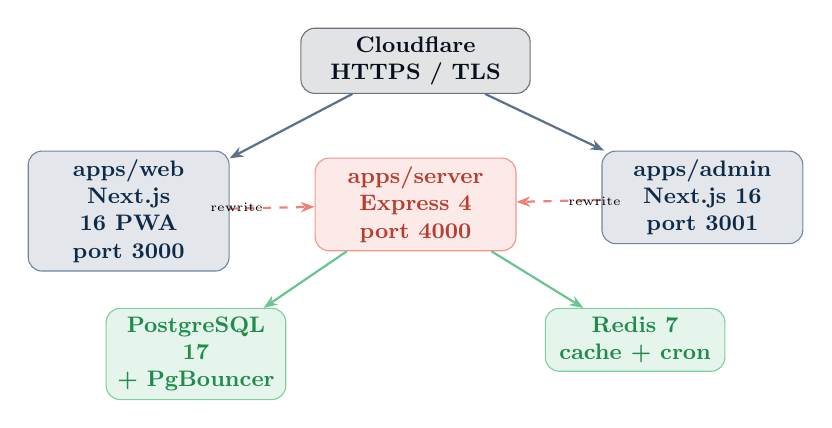
\begin{tikzpicture}[scale=0.9,transform shape,
  node distance=0.55cm and 1.0cm]

  \node[svc=mprimary!40!black,text width=3.0cm] (cf)
    {Cloudflare\\HTTPS / TLS};

  \node[svc=mprimary,below left=0.8cm and 1.0cm of cf,text width=2.6cm] (web)
    {apps/web\\Next.js 16 PWA\\port 3000};
  \node[svc=mprimary,below right=0.8cm and 1.0cm of cf,text width=2.6cm] (adm)
    {apps/admin\\Next.js 16\\port 3001};

  \node[svc=maccent,below=0.9cm of cf,text width=2.6cm] (srv)
    {apps/server\\Express 4\\port 4000};

  \node[svc=msuccess,below left=0.8cm and 0.4cm of srv,text width=2.3cm] (pg)
    {PostgreSQL 17\\+ PgBouncer};
  \node[svc=msuccess,below right=0.8cm and 0.4cm of srv,text width=2.3cm] (rd)
    {Redis 7\\cache + cron};

  \draw[arr=mprimary] (cf) -- (web);
  \draw[arr=mprimary] (cf) -- (adm);
  \draw[arr=maccent,dashed] (web) -- node[left,font=\tiny]{rewrite} (srv);
  \draw[arr=maccent,dashed] (adm) -- node[right,font=\tiny]{rewrite} (srv);
  \draw[arr=msuccess] (srv) -- (pg);
  \draw[arr=msuccess] (srv) -- (rd);
\end{tikzpicture}
\end{center}
\end{frame}

\begin{frame}[shrink=18]{技術堆疊}
\begin{columns}[T,onlytextwidth]
\begin{column}{0.48\textwidth}
  \begin{block}{前端}
    \begin{itemize}\small
      \item Next.js 16 + React 19（Turbopack）
      \item shadcn/ui（Base UI）+ Tailwind v4
      \item next-intl（zh-TW / en / ja）
      \item PWA：Service Worker + Manifest
    \end{itemize}
  \end{block}
  \begin{block}{後端}
    \begin{itemize}\small
      \item Express 4 + TypeScript
      \item Drizzle ORM + PostgreSQL 17 + PgBouncer
      \item Redis 7（快取 + 計數）
      \item Pino 結構化 JSON 日誌
    \end{itemize}
  \end{block}
\end{column}
\begin{column}{0.48\textwidth}
  \begin{block}{工具鏈 \& 部署}
    \begin{itemize}\small
      \item Bun 1 + Turborepo（Monorepo）
      \item Docker Compose（生產環境）
      \item Kubernetes + kind（本機叢集）
      \item Prometheus + Grafana + Loki
    \end{itemize}
  \end{block}
  \begin{block}{認證 \& 測試}
    \begin{itemize}\small
      \item 員工：JWT httpOnly cookie（8h）
      \item 管理員：UUID session（24h）
      \item Vitest + Supertest｜k6（1k VU）
    \end{itemize}
  \end{block}
\end{column}
\end{columns}
\end{frame}

\begin{frame}[shrink=5]{資料庫 ER 圖}
\begin{center}
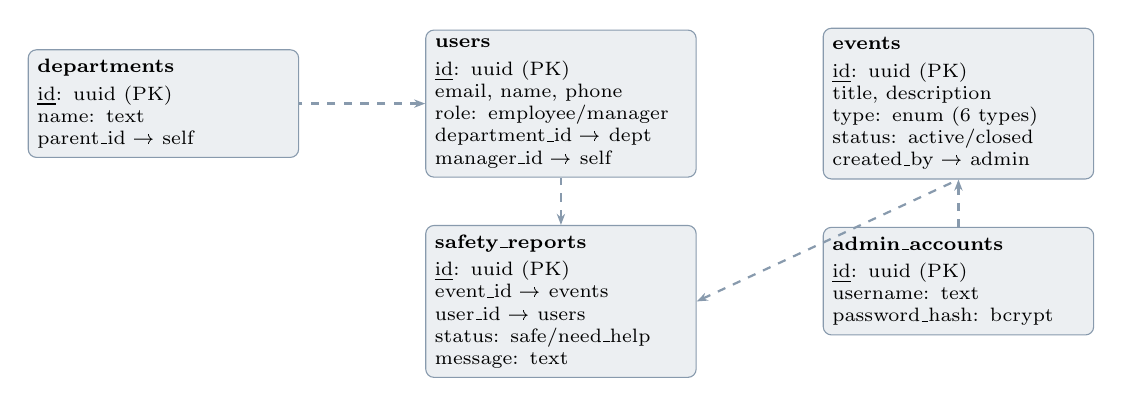
\begin{tikzpicture}[
  node distance=0.6cm and 1.6cm,
  tbl/.style={rectangle,rounded corners=3pt,draw=mprimary!50,
    fill=mprimary!8,text width=3.2cm,font=\scriptsize,align=left},
  fk/.style={{Stealth[length=4pt]}-,draw=mprimary!50,dashed,thick},
]
  \node[tbl] (dept) {%
    \textbf{departments}\\[2pt]
    \underline{id}: uuid (PK)\\
    name: text\\
    parent\_id \textrightarrow{} self};

  \node[tbl,right=of dept] (users) {%
    \textbf{users}\\[2pt]
    \underline{id}: uuid (PK)\\
    email, name, phone\\
    role: employee/manager\\
    department\_id \textrightarrow{} dept\\
    manager\_id \textrightarrow{} self};

  \node[tbl,right=of users] (events) {%
    \textbf{events}\\[2pt]
    \underline{id}: uuid (PK)\\
    title, description\\
    type: enum (6 types)\\
    status: active/closed\\
    created\_by \textrightarrow{} admin};

  \node[tbl,below=of users] (reports) {%
    \textbf{safety\_reports}\\[2pt]
    \underline{id}: uuid (PK)\\
    event\_id \textrightarrow{} events\\
    user\_id \textrightarrow{} users\\
    status: safe/need\_help\\
    message: text};

  \node[tbl,below=of events] (admin) {%
    \textbf{admin\_accounts}\\[2pt]
    \underline{id}: uuid (PK)\\
    username: text\\
    password\_hash: bcrypt};

  \draw[fk] (users.west) -- (dept.east);
  \draw[fk] (reports.north) -- (users.south);
  \draw[fk] (reports.east) -- (events.south);
  \draw[fk] (events.south) -- (admin.north);
\end{tikzpicture}
\end{center}
\vspace{-0.1cm}
{\scriptsize\textit{另有 department\_translations、event\_translations 兩張翻譯表支援 i18n}}
\end{frame}

\begin{frame}[shrink=12]{即時通訊 \& 快取設計}
\begin{columns}[T,onlytextwidth]
\begin{column}{0.52\textwidth}
  \begin{block}{SSE（Server-Sent Events）}
    \begin{itemize}\small
      \item \texttt{GET /api/sse}，text/event-stream
      \item 心跳每 25s，防止 idle proxy 斷線
      \item 依角色分流：
        \begin{itemize}\scriptsize
          \item \texttt{broadcastAll}：全體通知
          \item \texttt{broadcastToOversight}：主管
          \item \texttt{sendToManagerChain}：沿層上報
          \item \texttt{sendToUser}：個人推播
        \end{itemize}
      \item 事件型別：\texttt{event\_created},\\
        \texttt{report\_updated}, \texttt{reminder}...
    \end{itemize}
  \end{block}
\end{column}
\begin{column}{0.44\textwidth}
  \begin{block}{Redis 統計快取}
    \begin{itemize}\small
      \item \texttt{/api/events/:id/stats} 快取 \textbf{3 秒}
      \item 每次 report upsert \textrightarrow{} 主動 \texttt{DEL}
      \item 高峰並發查詢打快取，DB 壓力最小化
    \end{itemize}
  \end{block}
  \begin{block}{遞迴階層查詢}
    \begin{itemize}\small
      \item \texttt{users.manager\_id} 自我參考
      \item PostgreSQL \texttt{WITH RECURSIVE} CTE
      \item 單一 SQL 取得完整管理樹
    \end{itemize}
  \end{block}
\end{column}
\end{columns}
\end{frame}

\begin{frame}[shrink=12]{Kubernetes 部署架構}
\begin{columns}[T,onlytextwidth]
\begin{column}{0.50\textwidth}
  \begin{block}{Auto-scaling \& 高可用}
    \begin{itemize}\small
      \item \textbf{HPA}：2 \textrightarrow{} 10 pods，CPU 目標 70\%
      \item \textbf{滾動更新}：\texttt{maxUnavailable: 0}\\（新 Pod Ready 後才下線舊 Pod）
      \item \textbf{PDB}：\texttt{minAvailable: 1}\\防止 eviction 造成全停
      \item Health check：\texttt{/api/health}\\（liveness + readiness probe）
    \end{itemize}
  \end{block}
\end{column}
\begin{column}{0.46\textwidth}
  \begin{block}{服務發現}
    \begin{itemize}\small
      \item ClusterIP Service（server/postgres/redis）
      \item Ingress Nginx + TLS
      \item ConfigMap + Secret 管理環境變數
    \end{itemize}
  \end{block}
  \begin{block}{同源 Cookie 流程}
    \begin{center}\small
      \textbf{Browser} \textrightarrow{} \textbf{Next.js}
      \textrightarrow{} \textbf{Express API}
    \end{center}
    \vspace{2pt}
    \scriptsize
    瀏覽器帶 Cookie 至同源 Next.js；\\
    Next.js \texttt{rewrite} 轉發 API 請求至後端，\\
    Cookie 一路隨 Header 傳遞，無跨域問題。
  \end{block}
\end{column}
\end{columns}
\end{frame}

% ============================================================
\section{系統測試與驗證}
% ============================================================

\begin{frame}[shrink=25]{測試策略}
\begin{columns}[T,onlytextwidth]
\begin{column}{0.48\textwidth}
  \begin{block}{整合測試（Integration Test）}
    \begin{itemize}\small
      \item \textbf{Vitest} + \textbf{Supertest}
      \item 打真實 PostgreSQL + Redis（非 mock）
      \item \texttt{resetAndSeed()} 每個 suite 前重置
      \item \texttt{REMINDER\_JOB\_DISABLED=1} 禁排程
    \end{itemize}
  \end{block}
  \vspace{0.3cm}
  \begin{block}{覆蓋範圍}
    \begin{itemize}\small
      \item Auth（login / JWT verify）
      \item Events CRUD
      \item Reports（upsert / list）
      \item Stats（快取命中 / 刷新）
      \item Users / Departments CRUD
    \end{itemize}
  \end{block}
\end{column}
\begin{column}{0.48\textwidth}
  \begin{block}{負載測試（Load Test）}
    \begin{itemize}\small
      \item \textbf{k6}，1,000 VU 模擬同時回報
      \item Seed：\textbf{10,000 使用者}（SEED\_SCALE=load）
      \item 流程：登入 \textrightarrow{} 取得事件 \textrightarrow{} 回報 \textrightarrow{} 查詢統計
    \end{itemize}
  \end{block}
  \vspace{0.3cm}
  \begin{exampleblock}{實測結果（1k VU）}
    \begin{itemize}\small
      \item p95 回應時間 \textbf{109.8 ms}（SLO \textless{} 500 ms \textcolor{msuccess}{\cmark}）
      \item 錯誤率 \textbf{0.000\%}（SLO \textless{} 0.5\% \textcolor{msuccess}{\cmark}）
      \item 成功回報 \textbf{64,599 筆}，0 筆失敗
    \end{itemize}
  \end{exampleblock}
\end{column}
\end{columns}
\end{frame}

\begin{frame}[shrink=28]{壓力緩解機制}
\begin{columns}[T,onlytextwidth]
\begin{column}{0.48\textwidth}
  \begin{block}{資料層}
    \begin{itemize}\small
      \item \textbf{PgBouncer}：連線池，避免 DB 連線耗盡
      \item \textbf{Redis cache}：stats 3s TTL，QPS 大幅降低
      \item Report \textbf{upsert} 語意，避免重複寫入競爭
    \end{itemize}
  \end{block}
\end{column}
\begin{column}{0.48\textwidth}
  \begin{block}{運算層}
    \begin{itemize}\small
      \item \textbf{HPA}：CPU \textgreater{} 70\% 自動擴增至 10 pods
      \item \textbf{滾動更新}：測試期間零停機
      \item \textbf{SSE 心跳}：避免長連線積累 timeout
    \end{itemize}
  \end{block}
\end{column}
\end{columns}
\vspace{0.3cm}
\begin{exampleblock}{測試小結}
  \small
  整合測試（Vitest + Supertest）每個 suite 前 \texttt{resetAndSeed()}，確保隔離；
  負載測試 k6 1k VU 實測：p95 \textbf{109.8 ms}（SLO \textless{} 500ms）、錯誤率 \textbf{0.000\%}、成功回報 64,599 筆。
\end{exampleblock}
\end{frame}

% ============================================================
\section{維運與可靠性}
% ============================================================

\begin{frame}[shrink=12]{可觀測性堆疊}
\begin{columns}[T,onlytextwidth]
\begin{column}{0.55\textwidth}
  \begin{block}{自訂 Prometheus Metrics（10 項）}
    \renewcommand{\arraystretch}{1.0}
    \begin{tabular}{ll}
    \scriptsize\texttt{http\_requests\_total}          & \scriptsize 請求計數 \\
    \scriptsize\texttt{http\_request\_duration\_seconds}& \scriptsize 延遲直方圖 \\
    \scriptsize\texttt{sse\_active\_connections}       & \scriptsize 即時連線數 \\
    \scriptsize\texttt{report\_submit\_total}           & \scriptsize 回報次數 \\
    \scriptsize\texttt{reminder\_emails\_total}         & \scriptsize 提醒郵件 \\
    \scriptsize\texttt{stats\_cache\_hits/misses\_total}& \scriptsize Redis 命中/miss \\
    \scriptsize\texttt{active\_events\_total}           & \scriptsize 進行中事件 \\
    \scriptsize\texttt{unreported\_users\_total}        & \scriptsize 未回報人數 \\
    \end{tabular}
  \end{block}
\end{column}
\begin{column}{0.41\textwidth}
  \begin{block}{Grafana Dashboards（3 張）}
    \begin{itemize}\small
      \item \textbf{API Overview}：QPS / p95 / 錯誤率
      \item \textbf{Business Metrics}：回報率、SSE、事件狀態
      \item \textbf{Infrastructure}：CPU、記憶體、DB 連線池
    \end{itemize}
  \end{block}
  \begin{block}{Loki + Promtail}
    \begin{itemize}\small
      \item Pino JSON 結構化日誌
      \item label：service / level
      \item LogQL 查詢慢請求 / 錯誤
    \end{itemize}
  \end{block}
\end{column}
\end{columns}
\end{frame}

\begin{frame}[shrink=15]{告警規則與可靠性設計}
\begin{columns}[T,onlytextwidth]
\begin{column}{0.50\textwidth}
  \begin{alertblock}{Prometheus 告警規則（3 條）}
    \begin{itemize}\small
      \item \textbf{HighErrorRate}：5 分鐘錯誤率 \textgreater{} 1\%
      \item \textbf{HighP95Latency}：p95 延遲 \textgreater{} 500 ms
      \item \textbf{SSEConnectionDrop}：連線數驟降偵測
    \end{itemize}
  \end{alertblock}
  \vspace{0.2cm}
  \begin{block}{零停機部署}
    \begin{itemize}\small
      \item \texttt{maxUnavailable: 0}，PDB \texttt{minAvailable: 1}
      \item \texttt{/api/health} liveness + readiness probe
    \end{itemize}
  \end{block}
\end{column}
\begin{column}{0.46\textwidth}
  \begin{block}{自我修復}
    \begin{itemize}\small
      \item Docker \texttt{restart: unless-stopped}
      \item K8s Pod crash \textrightarrow{} 自動重啟
      \item HPA 自動擴縮（2--10 pods）
    \end{itemize}
  \end{block}
  \begin{block}{服務分層可靠性}
    \begin{itemize}\small
      \item PgBouncer：DB 連線數可控
      \item Reminder cron：最多 3 次 / (event, user)
      \item Redis TTL：自動清理 stale cache
    \end{itemize}
  \end{block}
\end{column}
\end{columns}
\end{frame}

% ── Summary ─────────────────────────────────────────────────
\begin{frame}[shrink=15]{總結}
\begin{center}
  {\Large\bfseries 護你安 HuYouAn}\\[0.4cm]
  {\normalsize 以雲原生架構實現企業員工緊急安全回報系統}
\end{center}
\vspace{0.3cm}
\begin{columns}[T,onlytextwidth]
\begin{column}{0.24\textwidth}
  \begin{block}{\centering 需求轉換}
    \centering\small 7 項 User Story\\全數實作
  \end{block}
\end{column}
\begin{column}{0.24\textwidth}
  \begin{block}{\centering 架構設計}
    \centering\small Monorepo + K8s\\HPA 自動擴縮
  \end{block}
\end{column}
\begin{column}{0.24\textwidth}
  \begin{block}{\centering 系統測試}
    \centering\small 整合 + k6 1k VU\\p95 109 ms / 錯誤率 0\%
  \end{block}
\end{column}
\begin{column}{0.24\textwidth}
  \begin{block}{\centering 維運可靠}
    \centering\small Prometheus / Grafana\\零停機部署
  \end{block}
\end{column}
\end{columns}
\vspace{0.4cm}
\begin{center}
  {\large\bfseries\color{mprimary} 謝謝聆聽，歡迎提問}\\[0.3cm]
  \small
  \textcolor{mprimary!60}{\textbf{Demo}} \enspace
  \texttt{\small https://cloud-native-final-project.ntu-bilab.com}\\[0.1cm]
  \textcolor{mprimary!60}{\textbf{GitHub}} \enspace
  \texttt{\small https://github.com/c0dypeng/cloud-native-final-project}
\end{center}
\end{frame}

\end{document}
